\documentclass[12pt,titlepage]{article}
\usepackage[margin=1.25in]{geometry}
\usepackage{graphicx,amsmath,minted}

%% Variables definition
\newcommand{\vSubject}{Computer Networking}
\newcommand{\vSubtitle}{GNS3}
\newcommand{\vName}{Dicha Zelianivan Arkana}
\newcommand{\vNIM}{2241720002}
\newcommand{\vClass}{2i}
\newcommand{\vDepartment}{Information Technology}
\newcommand{\vStudyProgram}{D4 Informatics Engineering}

%% [START] Tikz related stuff
\usepackage{tikz}
\usetikzlibrary{svg.path,calc,shapes.geometric,shapes.misc}
\tikzstyle{terminator} = [rectangle, draw, text centered, rounded corners = 1em, minimum height=2em]
\tikzstyle{preparation} = [chamfered rectangle, chamfered rectangle sep=0.75em, draw, text centered, minimum height = 2em]
\tikzstyle{process} = [rectangle, draw, text centered, minimum height=2em]
\tikzstyle{decision} = [diamond, aspect=2, draw, text centered, minimum height=2em]
\tikzstyle{data}=[trapezium, draw, text centered, trapezium left angle=60, trapezium right angle=120, minimum height=2em]
\tikzstyle{connector} = [line width=0.25mm,->]
%% [END] Tikz related stuff

%% [START] Fancy header related stuff
\usepackage{fancyhdr}
\pagestyle{fancy}
\setlength{\headheight}{15pt} % compensate fancyhdr style
\fancyhead{}
\fancyfoot{}
\fancyfoot[L]{\thepage}
\fancyfoot[R]{\textit{\vSubject - \vSubtitle}}
\renewcommand{\footrulewidth}{0.4pt}% default is 0pt, overline for footer
%% [END] Fancy header related stuff

%% [START] Custom tabular command related stuff
\usepackage{tabularx}
\newcommand{\details}[2]{
    #1 & #2  \\
}
%% [END] Custom tabular command related stuff

%% [START] Figure related stuff
\newcommand{\image}[3][1]{
    \begin{figure}[h]
        \centering
        \includegraphics[#1]{#2}
        \caption{#3}
        \label{#3}
    \end{figure}
}
%% [END] Figure related stuff

\begin{document}
\begin{titlepage}
    \centering
    \vfill
    {\bfseries\LARGE
        \vSubject\\
        \vskip0.25cm
        \vSubtitle
    }
    \vfill
    
\includegraphics[width=6cm]{images/polinema-logo.png}
    \vfill
    {
        \textbf{Name}\\
        \vName\\
        \vskip0.5cm
        \textbf{NIM}\\
        \vNIM\\
        \vskip0.5cm
        \textbf{Class}\\
        \vClass\\
        \vskip0.5cm
        \textbf{Department}\\
        \vDepartment\\
        \vskip0.5cm
        \textbf{Study Program}\\
        \vStudyProgram
    }
\end{titlepage}

\section{GNS3 Installation}

I use Linux, so the way I installed it is going to be different from Windows or MacOS. I installed it
using the \texttt{pip3} package manager. The command to install it is as follows:

\begin{minted}[fontsize=\footnotesize]{bash}
    pip3 install gns3-gui==2.2.17 PyQt5 psutil
\end{minted}

The \texttt{PyQt5} and \texttt{psutil} are the dependency packages that is needed by GNS3. After
that, the GNS3 app should appear in the application menu like shown below.

\begin{center}
    
\includegraphics[height=4cm]{./images/gns-application-list.png}
\end{center}

If we click on the GNS3 app, the GNS3 GUI will appear like shown below.

\begin{center}
    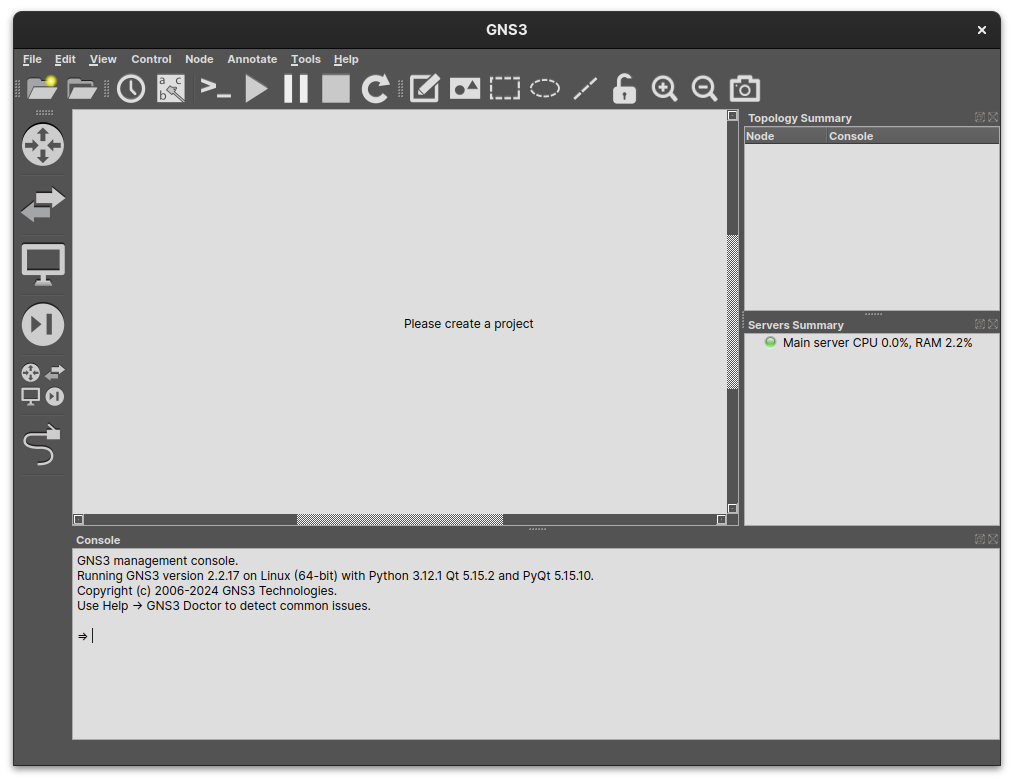
\includegraphics[width=0.8\textwidth]{./images/gns3-gui.png}
\end{center}

\section{OpenVPN Installation}

The OpenVPN installation is not needed since my Linux which is Fedora comes with
OpenVPN pre-installed. We can check it by running the following command.

\begin{minted}[fontsize=\footnotesize]{bash}
    openvpn --version
\end{minted}

The output should look as follow:

\begin{center}
    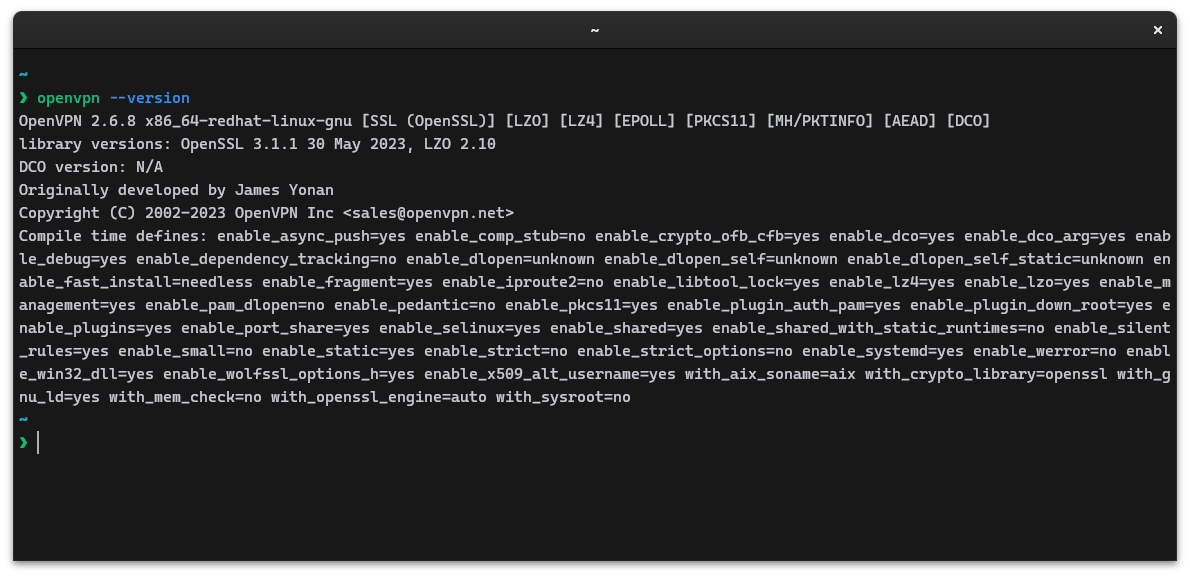
\includegraphics[width=0.8\textwidth]{./images/openvpn-version.png}
\end{center}

To connect to the OpenVPN server, we need to have the \texttt{.ovpn} file
and then connect it using the following command

\begin{minted}[fontsize=\footnotesize]{bash}
    openvpn --config TI2I08.ovpn
\end{minted}

It should output the following message if the connection is successful.

\begin{center}
    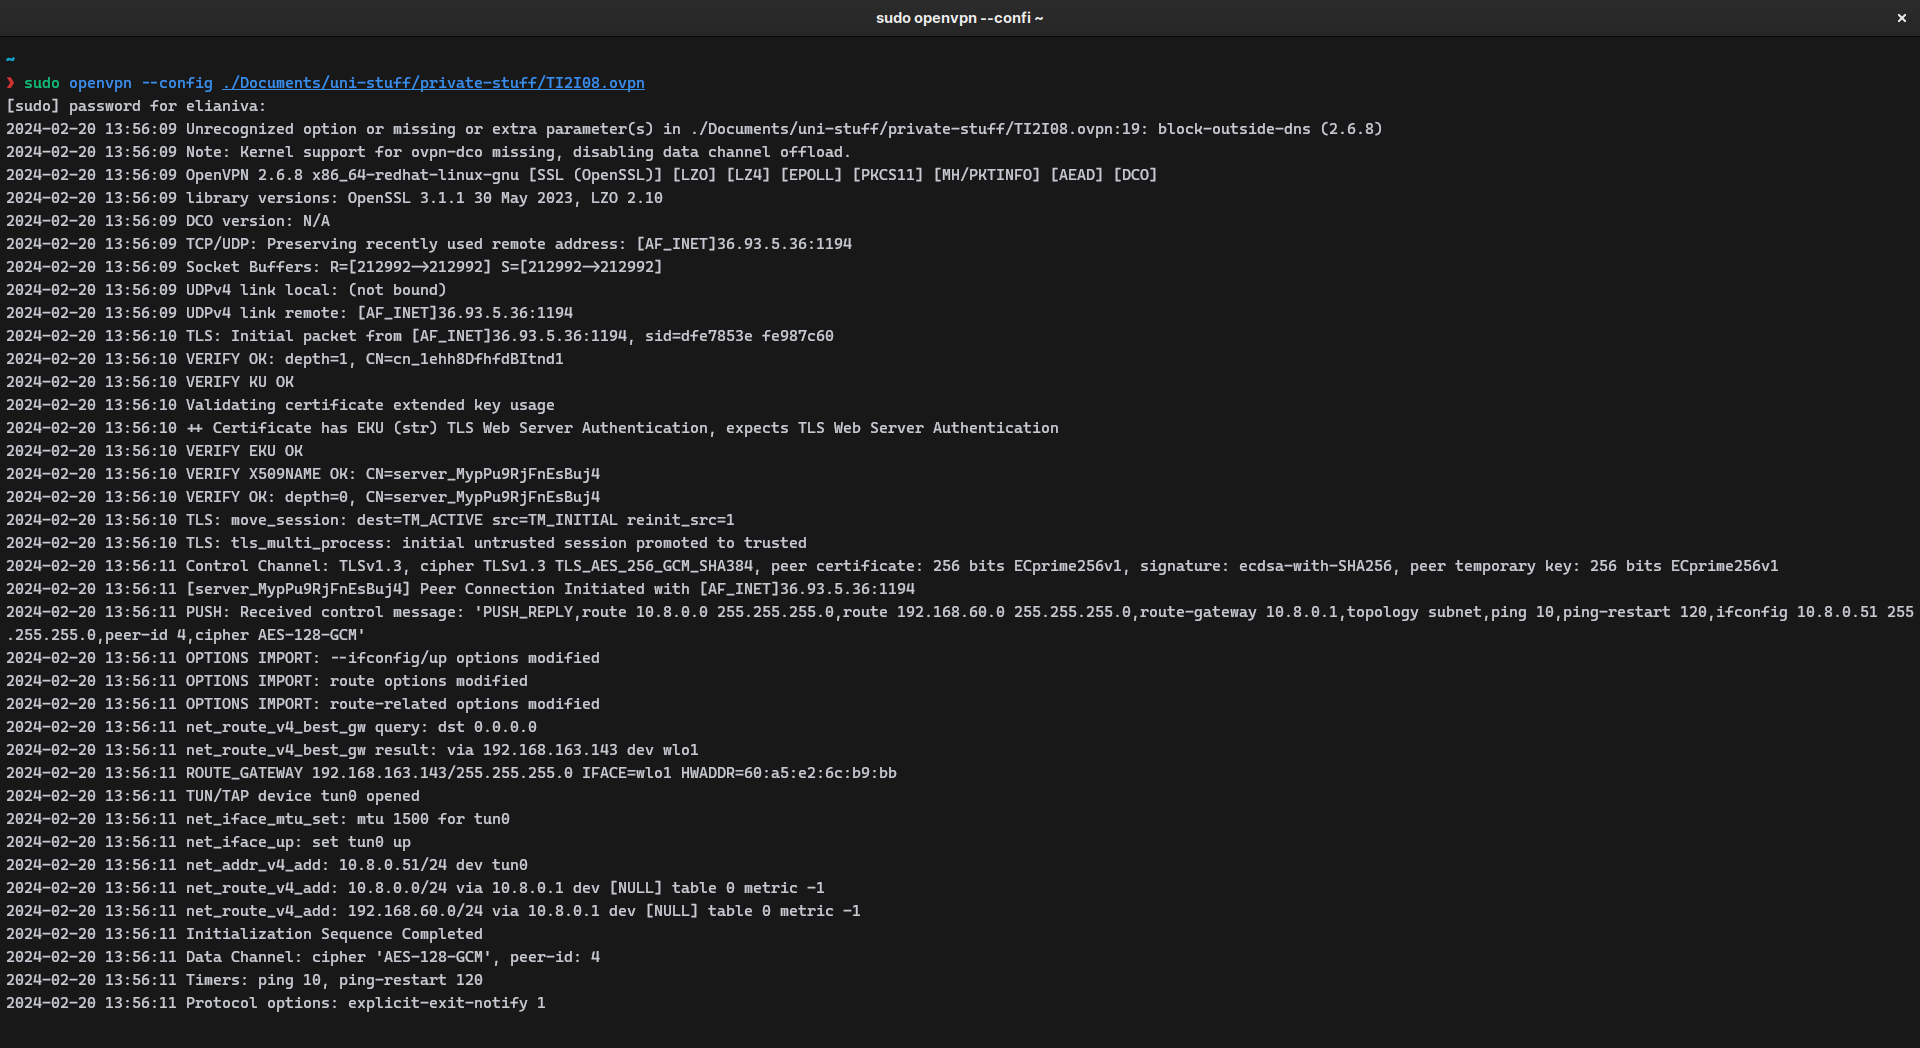
\includegraphics[width=0.8\textwidth]{./images/openvpn-connected.png}
\end{center}

\end{document}

